%% Tex spellcheck = fr_FR
\chapter{Chapter 5 : Final Tic-Tac-Toe hardware design}

Now that we found the best coil design, we can make a full matrix of coils to move the magnet in a 2D space. We will use the square coils with sub-coils. we will also need a driver circuit power the matrix of coils individually.

\section{Choice of layout}

We want to make a matrix big enough to play Tic-Tac-Toe. This means that we need at least 3x3 usable cells plus some side coils to hold the non placed pieces. So in the end we need a 5x4 usable matrix of coils. But as we describe in the next section, we also need intermediate buses to avoid attracting the wrong magnets. This means that for each usable cell, we need a triple bus for rows and columns.


\begin{figure}[H]
	\centering
	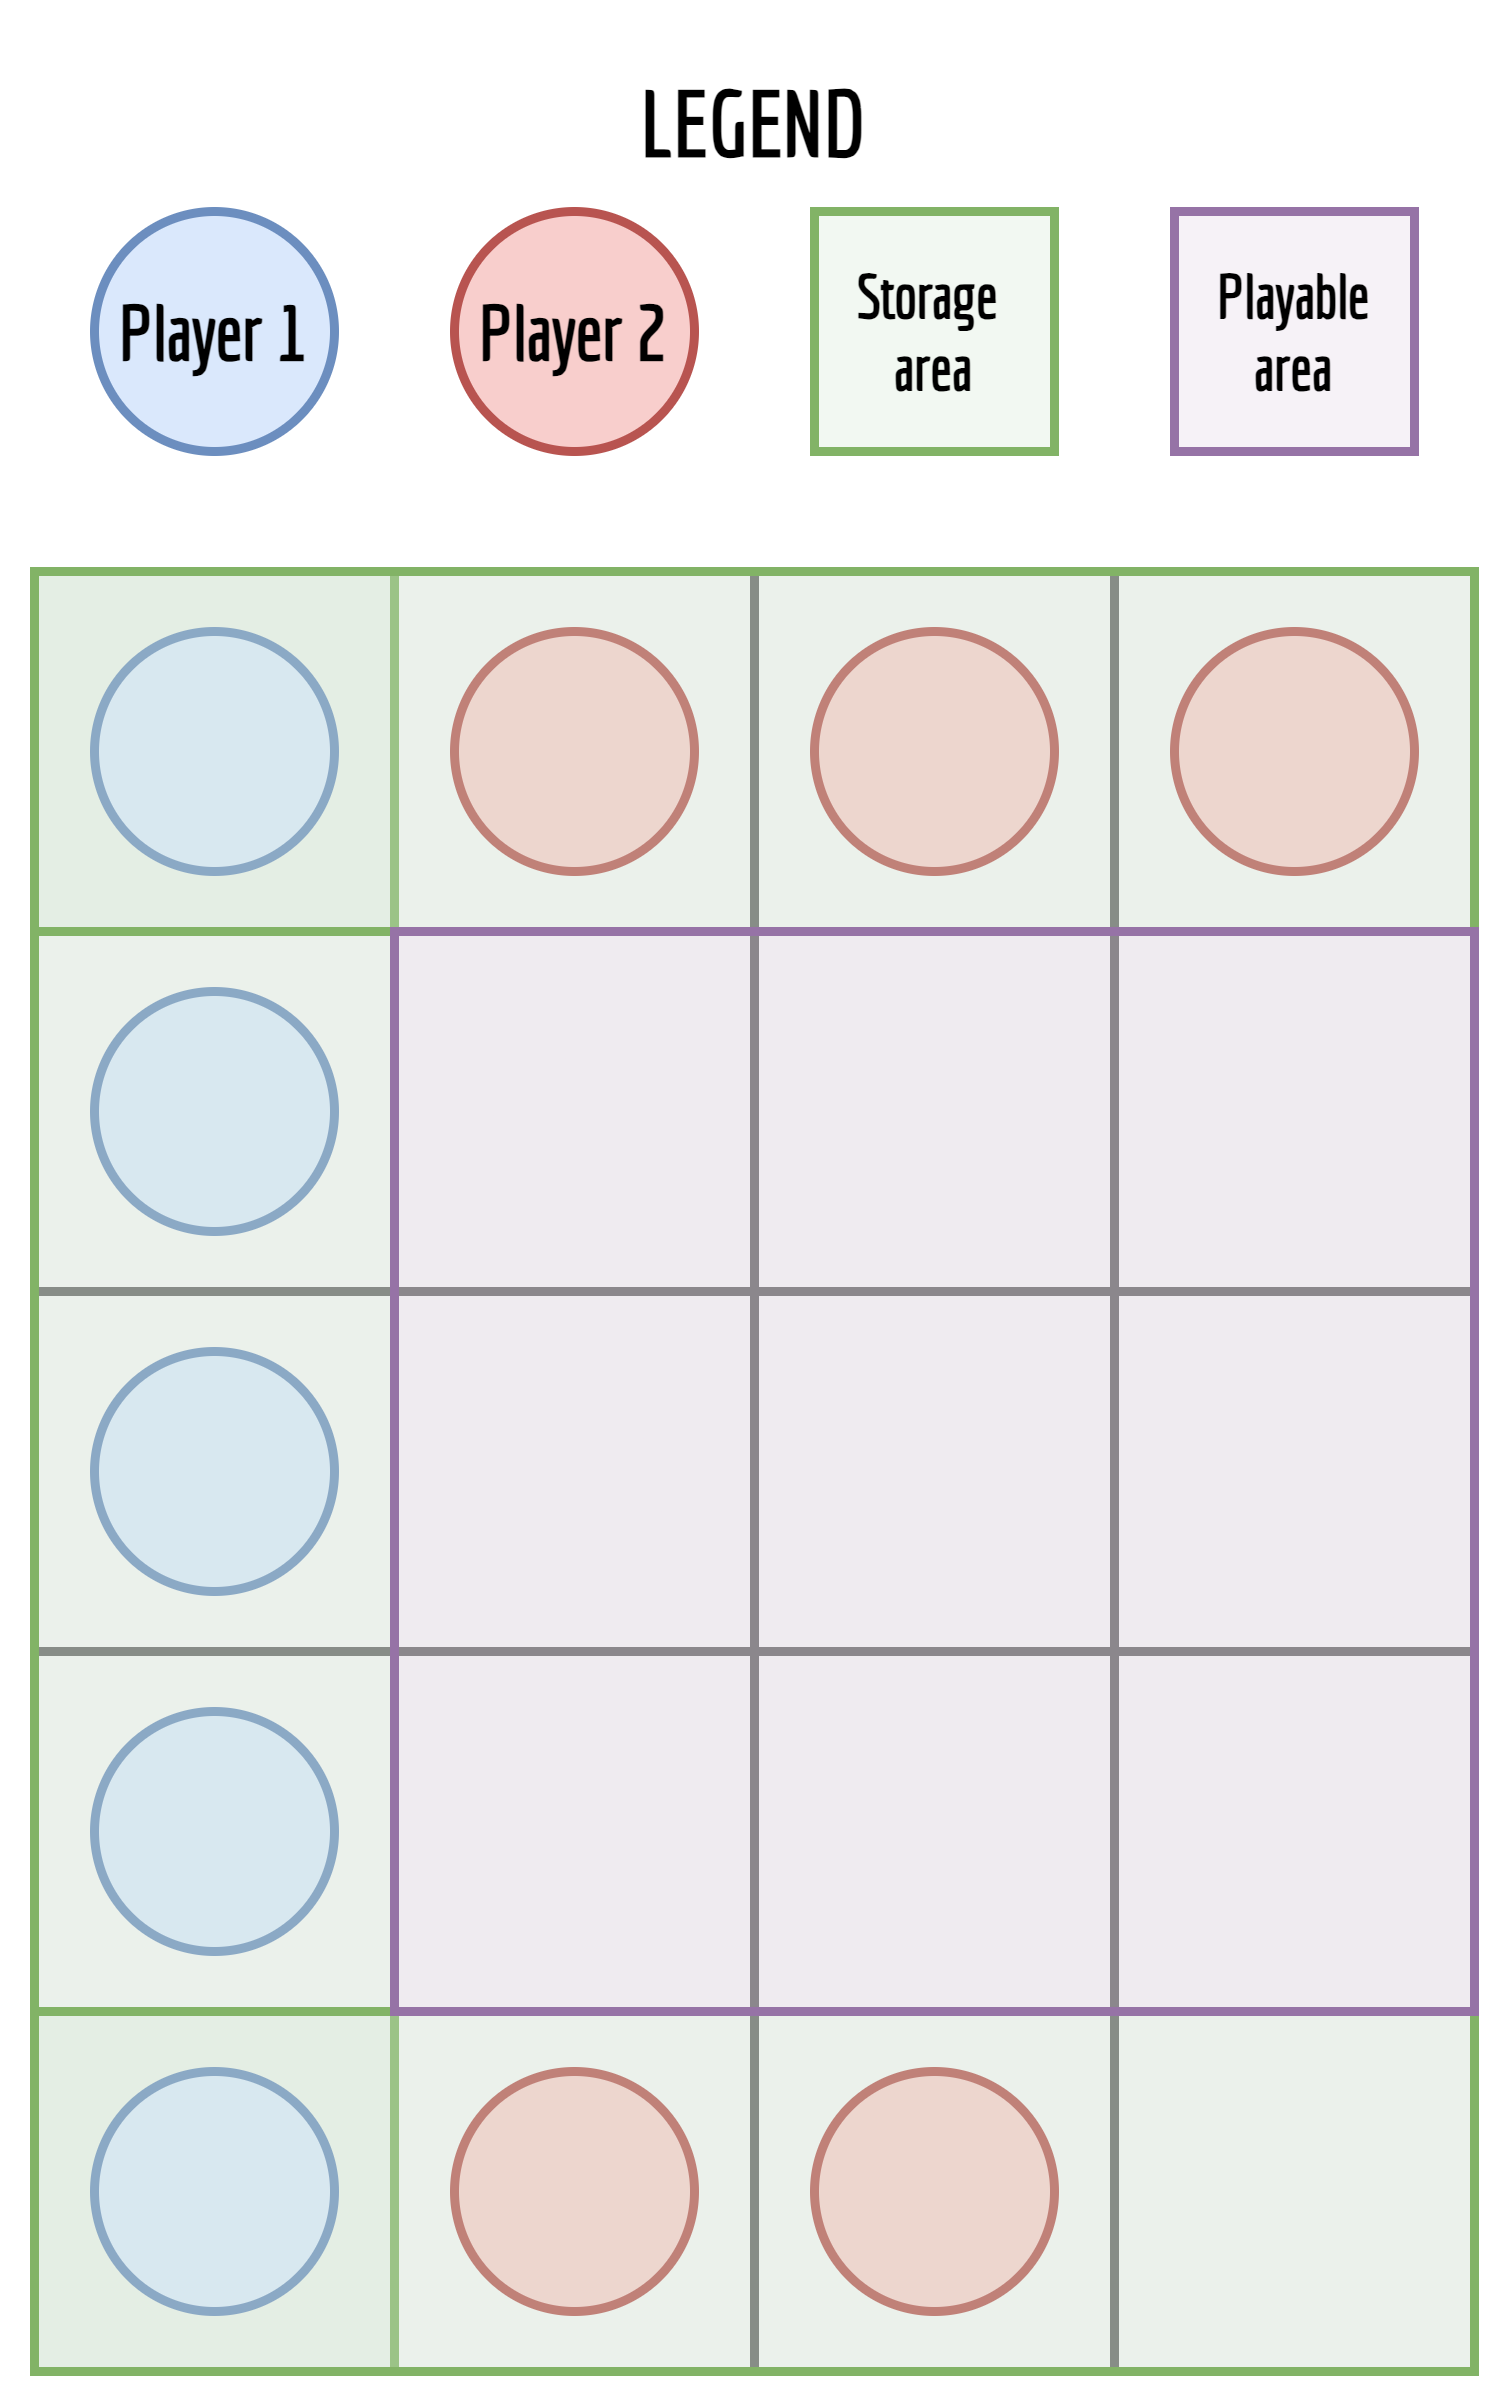
\includegraphics[width=0.5\linewidth]{playable_zones.png}
	\caption[Description of zones for tic-tac-toe]{Description of zones for tic-tac-toe}
	\label{fig:playable_zones}
\end{figure}


\subsection{Magnet buses}

Since the design can attract magnets from any directions, we need intermediate buses or routes to avoid attracting the wrong magnets.

The issue is a single bus would not be enough since activation a coil on the bus with magnets on both sides would attract both magnets.

\begin{figure}[H]
	\centering
	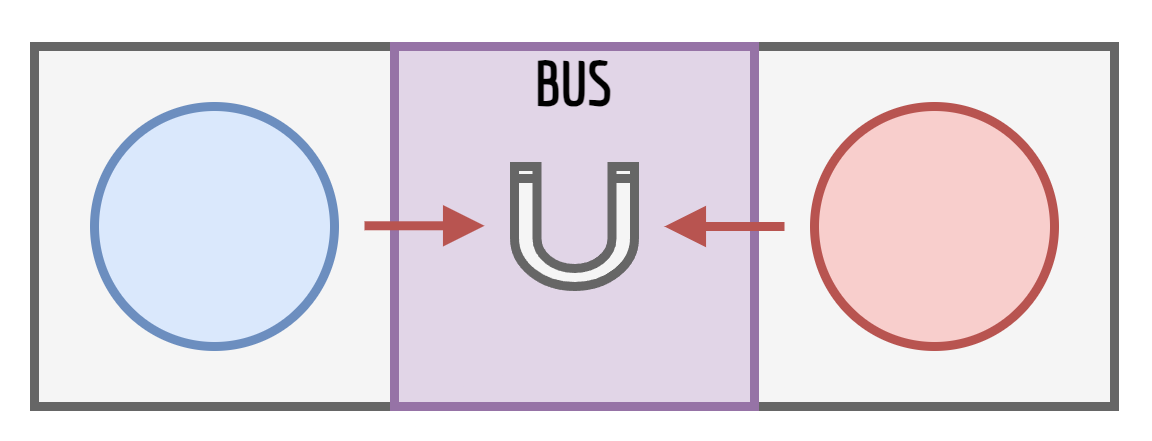
\includegraphics[width=0.8\linewidth]{single_bus.png}
	\caption[Magnet single bus]{Magnet single bus}
	\label{fig:single_bus}
\end{figure}

\newpage

A dual bus would still not be enough since when moving from one cell to another, we could come across situations where the path requires to activate a coil on the bus with magnets on both sides.

\begin{figure}[H]
	\centering
	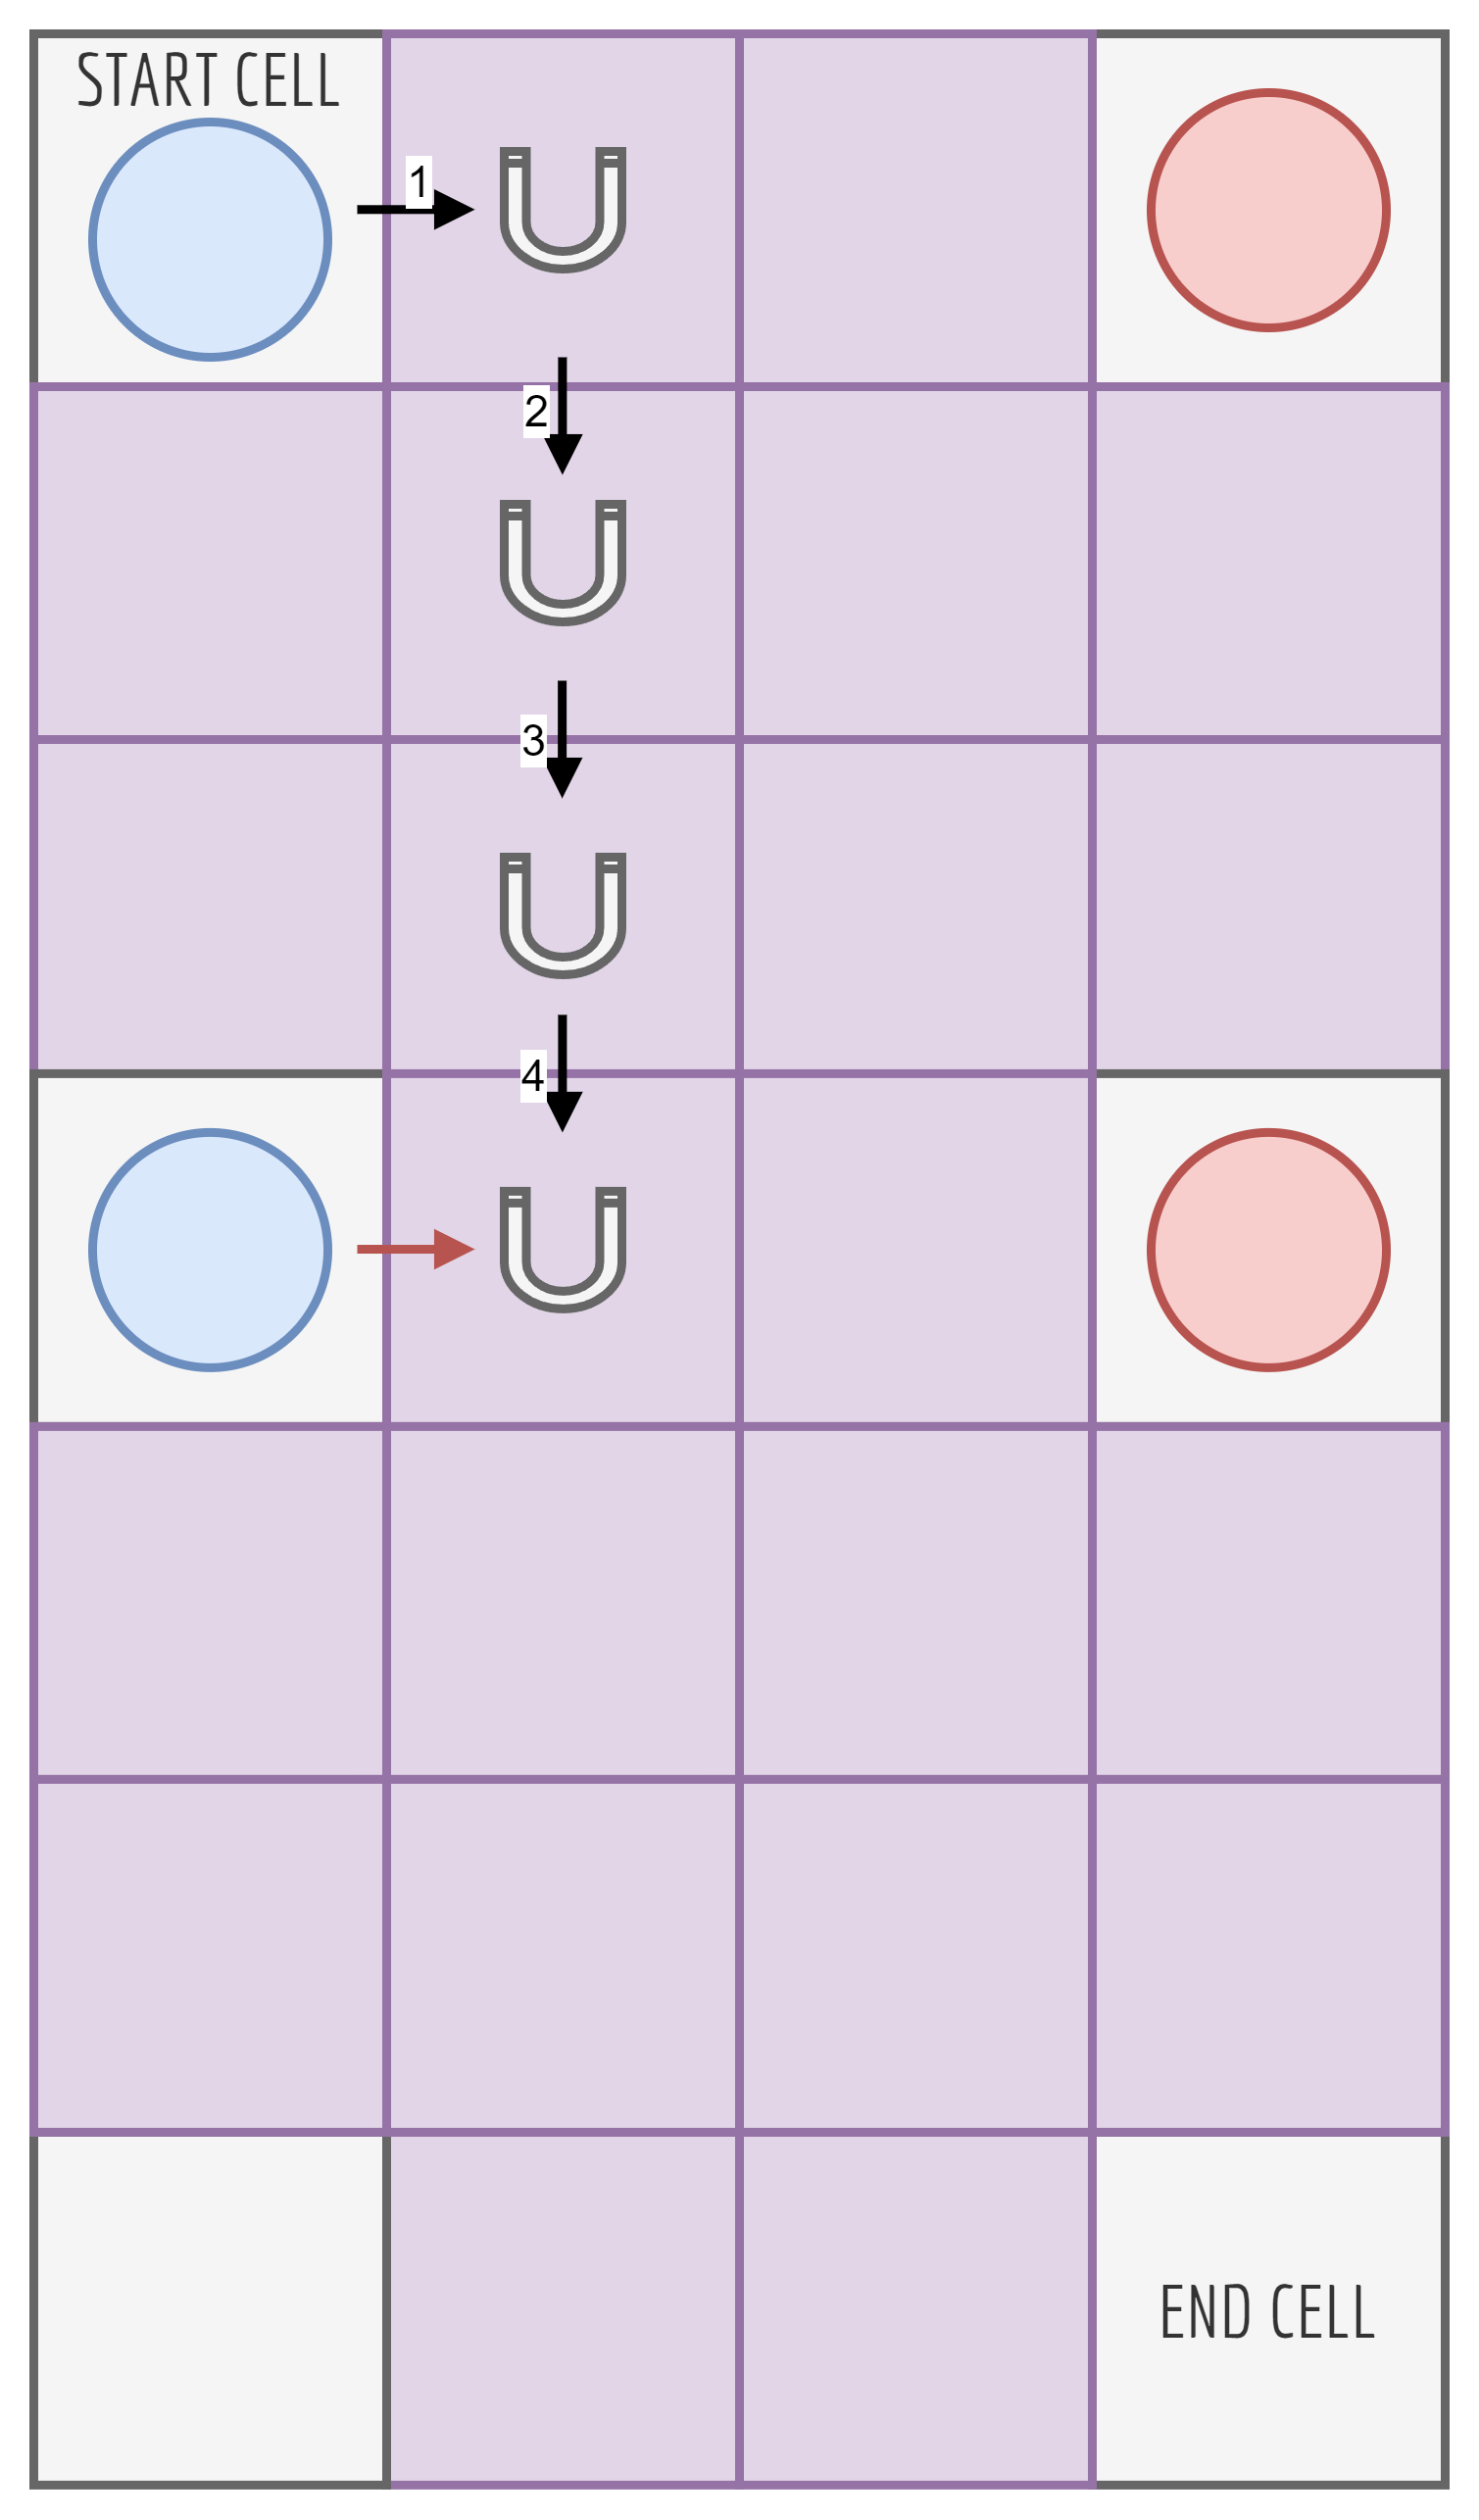
\includegraphics[width=0.7\linewidth]{double_bus.png}
	\caption[Magnet dual bus]{Magnet dual bus}
	\label{fig:double_bus.png}
\end{figure}

\newpage

The solution would be to have a triple bus system. This way we go onthe middle of the bus to move anywhere without attracting the wrong magnets.

\begin{figure}[H]
	\centering
	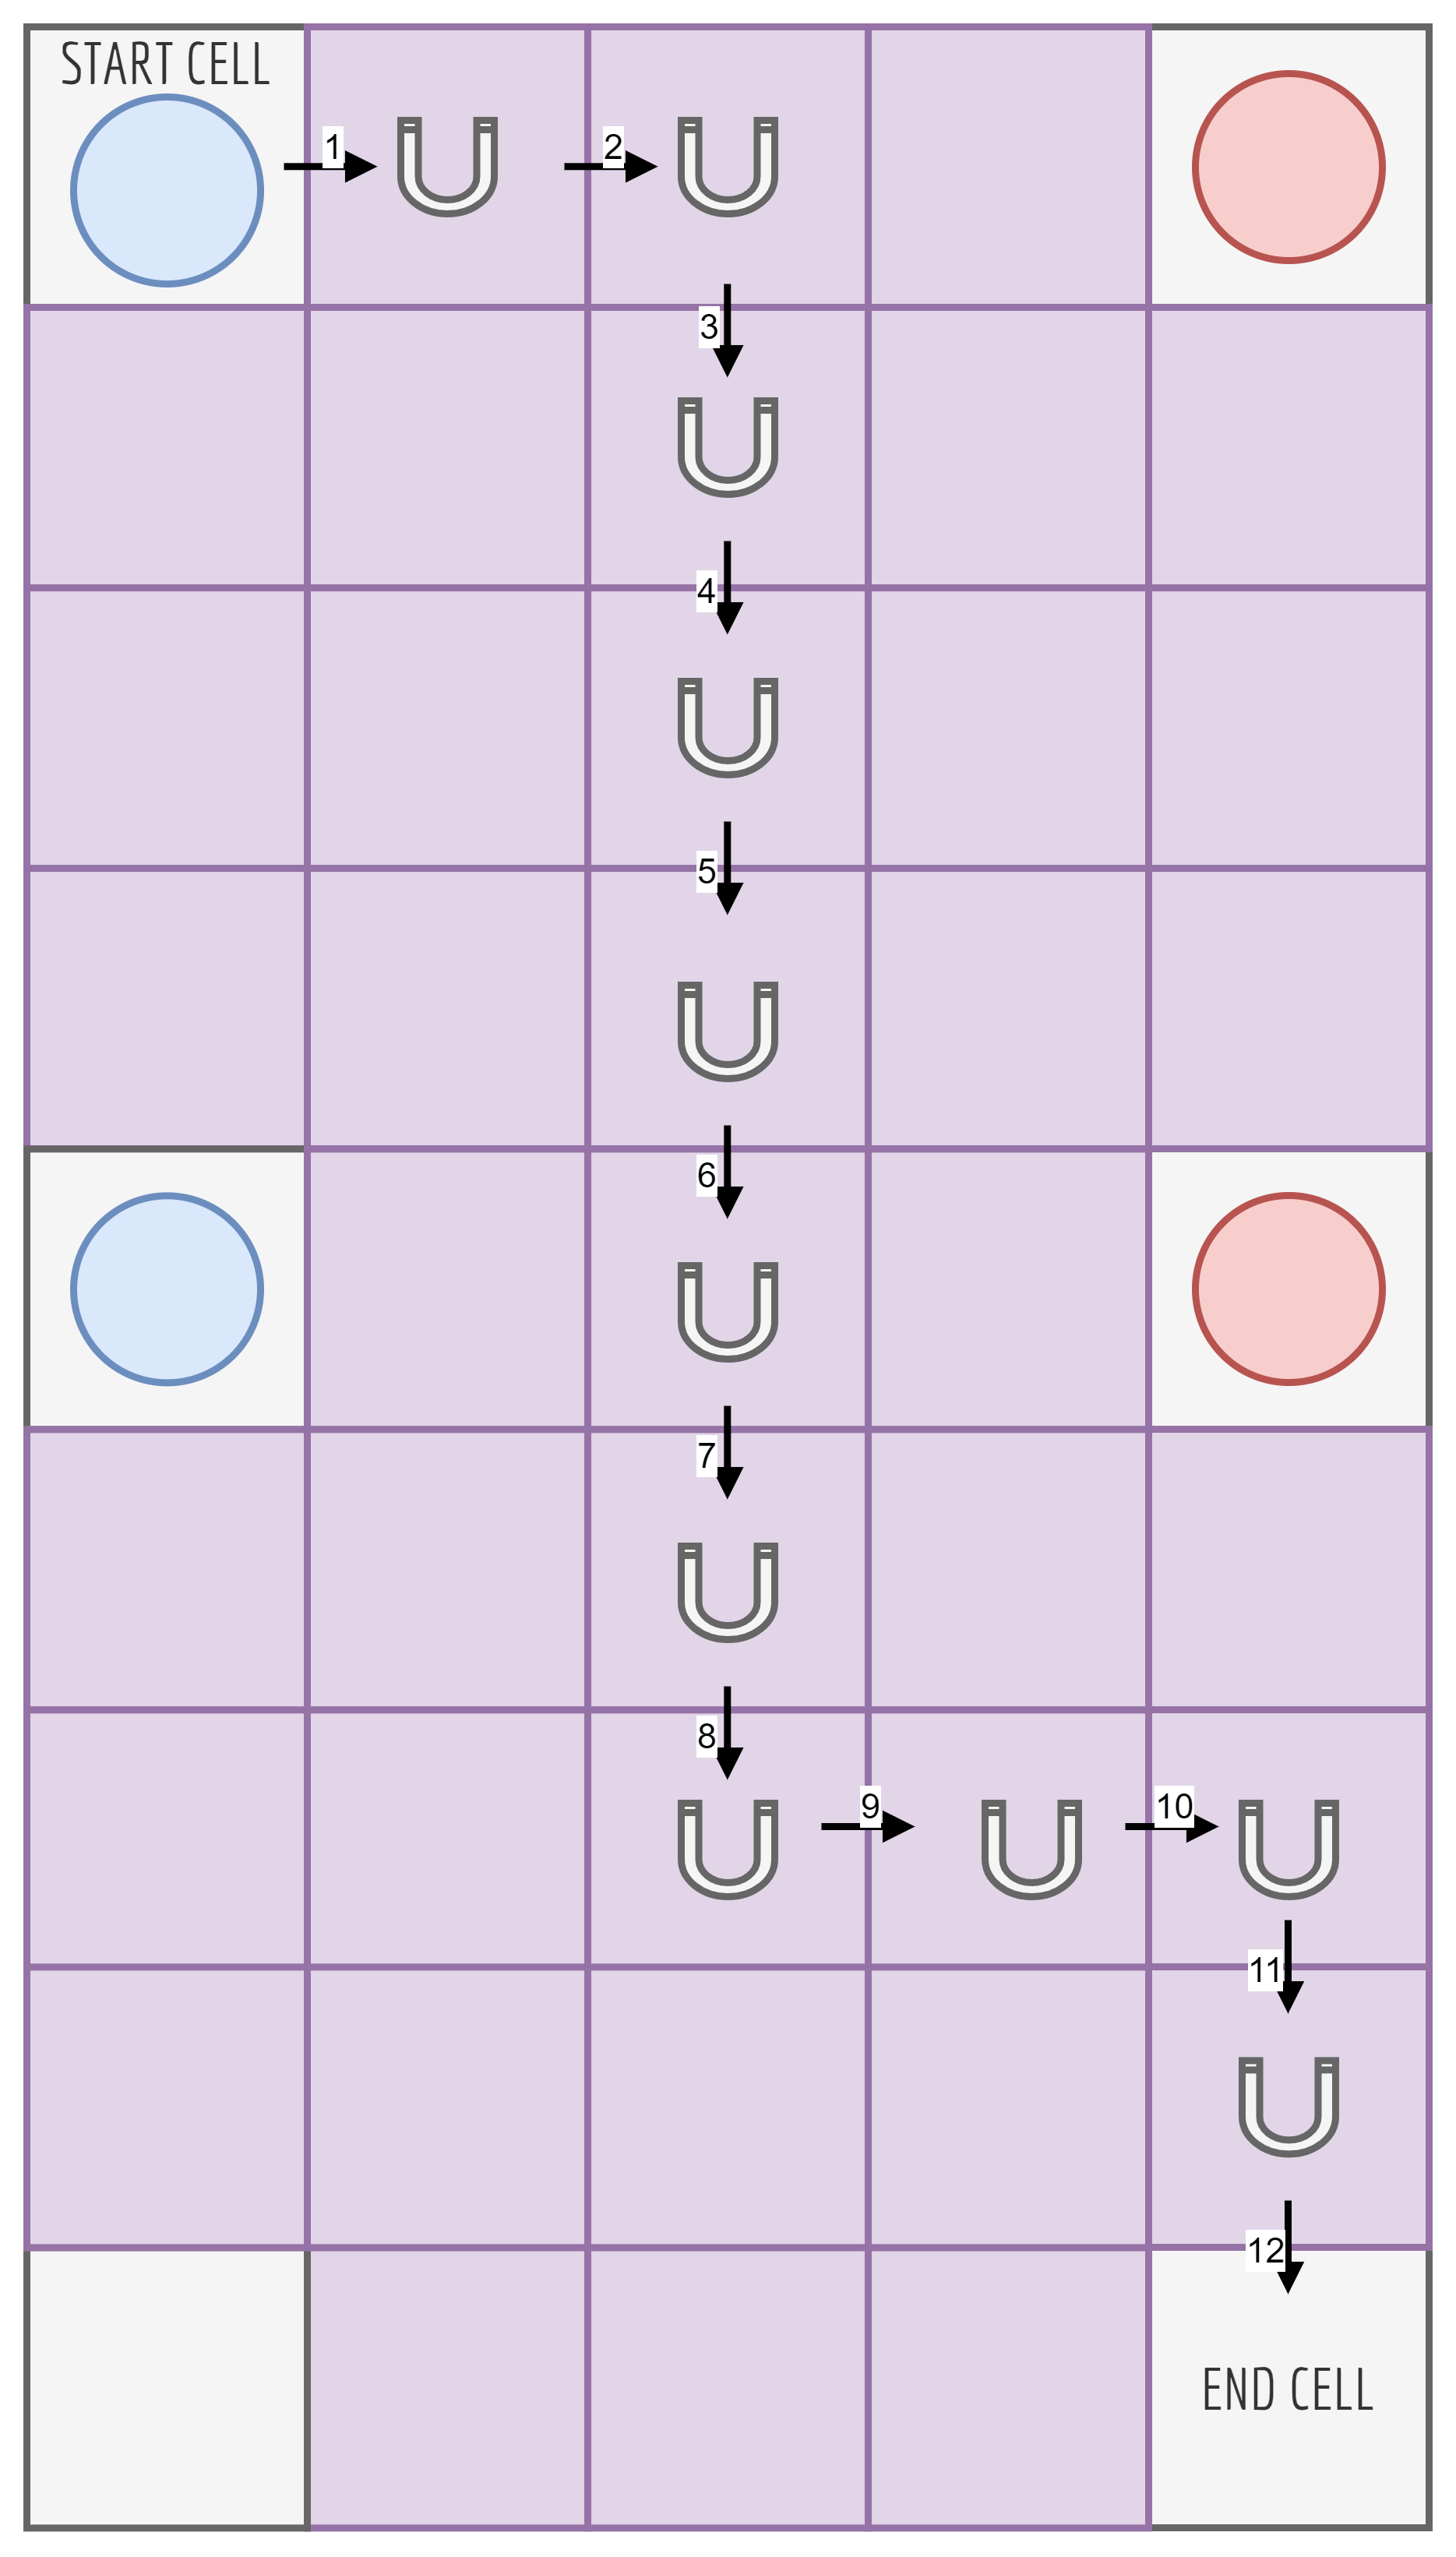
\includegraphics[width=0.7\linewidth]{triple_bus.png}
	\caption[Magnet triple bus]{Magnet triple bus}
	\label{fig:triple_bus}
\end{figure}


\begin{figure}[H]
	\centering
	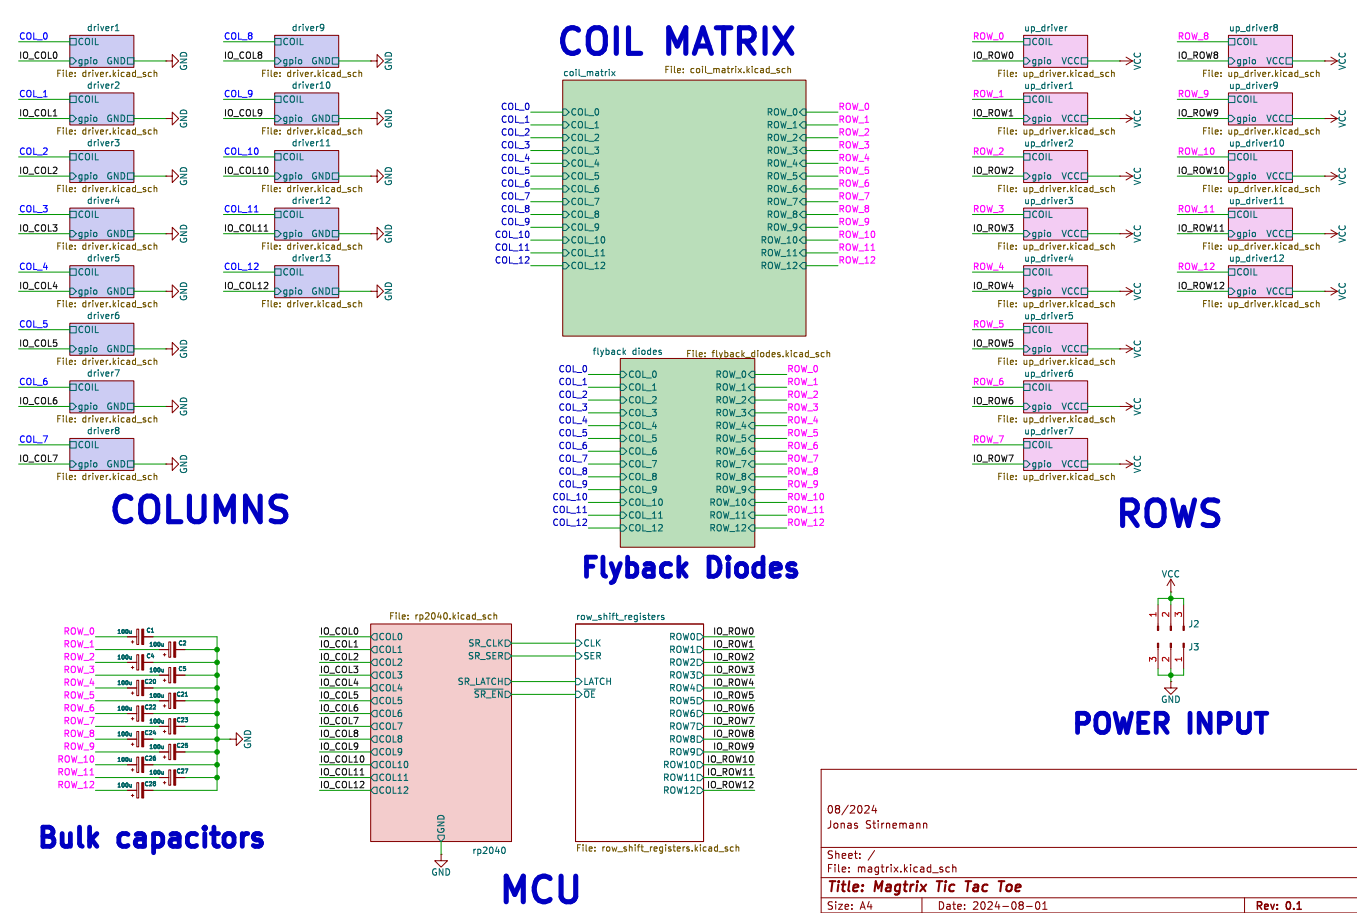
\includegraphics[width=1.4\linewidth, angle=90]{general_schematics.png}
	\caption[General schematics of final design]{General schematics of final design}
	\label{fig:general_schematics}
\end{figure}


\section{Driver circuit}

Now that we have a matrix of coils, it would take space, time and money to have a driver circuit for each coil. We will use a row and column driving method. This means that each coil will be connected to a row and a column. We will then activate the row and column to activate the coil. This way we can activate any coil in the matrix by activating the corresponding row and column. Each row is driven by a PMOS transistor, pulling one side of the coil to VCC and each column is driven by a NMOS transistor, pulling the other side of the coil to GND.

\begin{figure}[H]
	\centering
	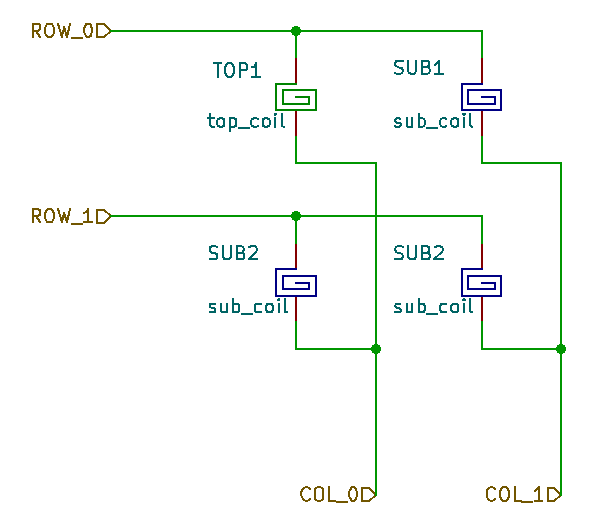
\includegraphics[width=0.8\linewidth]{row_col_drive.png}
	\caption[Matrix driving concept]{Matrix driving concept}
	\label{fig:matrix_concept}
\end{figure}

\newpage

This means that each coil is driven by the equivalent of this schematics.

\begin{figure}[H]
	\centering
	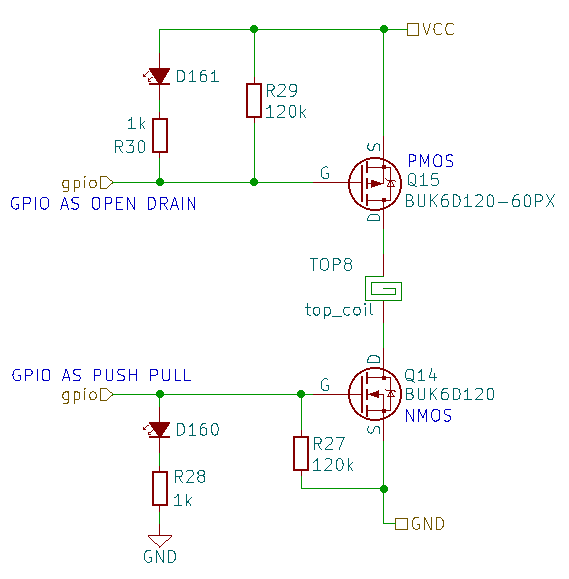
\includegraphics[width=0.6\linewidth]{driver_mos.png}
	\caption[Equivalent Dual mos driver circuit]{Equivalent Dual mos driver circuit}
	\label{fig:driver_mos}
\end{figure}

\section{Kicad scripting}

I've tried to leverage the power of scripting in Kicad and create three simple scripts. They need to run with the Kicad's python instance since they use the Kicad API.

\subsection{Footprint generation}
One of them to create the footprint of the coil itself by specifying the parameters of the coils:

\begin{itemize}
	\item The traces width,
	\item The spacing between traces
	\item The side of the square
\end{itemize}

\begin{figure}[H]
	\centering
	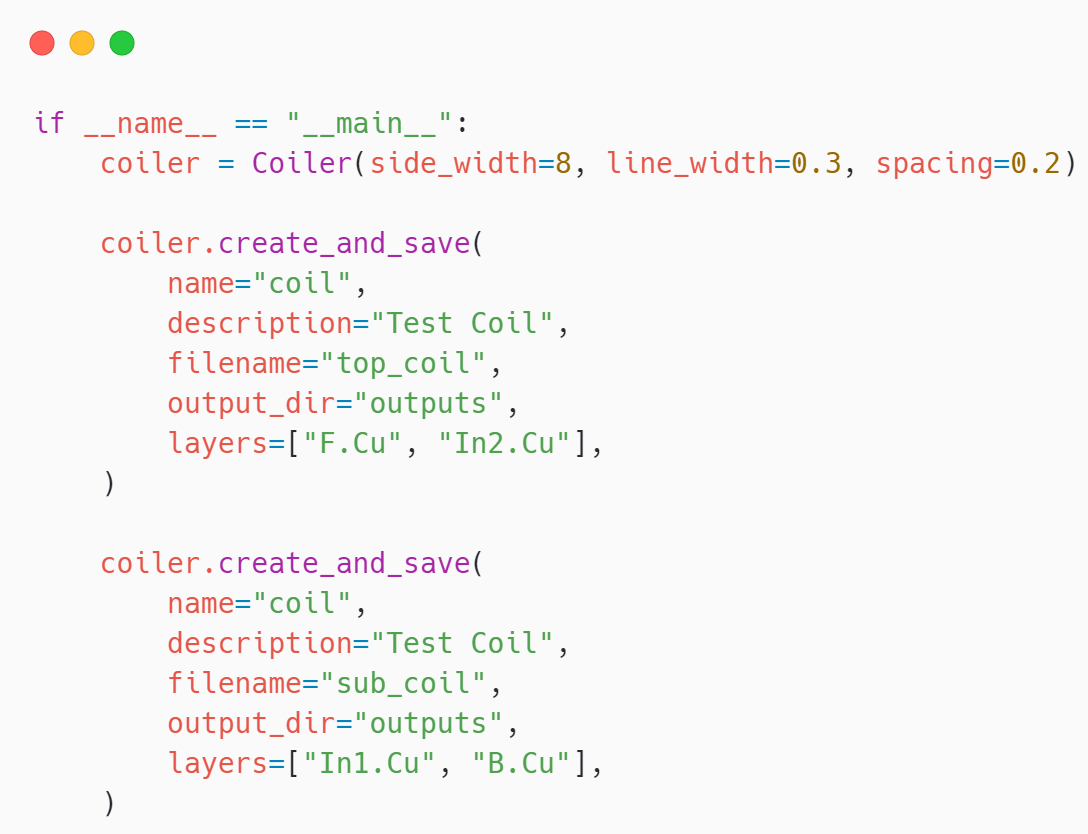
\includegraphics[width=0.8\linewidth]{code_footprint.png}
	\caption[Code to generate Kicad square footprint]{Code to generate Kicad square footprint}
	\label{fig:coil_footprint}
\end{figure}

\subsection{Schematic generation}
Now that we have the footprint, we want to generate a matrix of coils in the schematic. For that we need to create a blank schematics and add and configure 2 coils. Then the script will duplicate the coils and connect them to the rows and columns.

\begin{figure}[H]
	\centering
	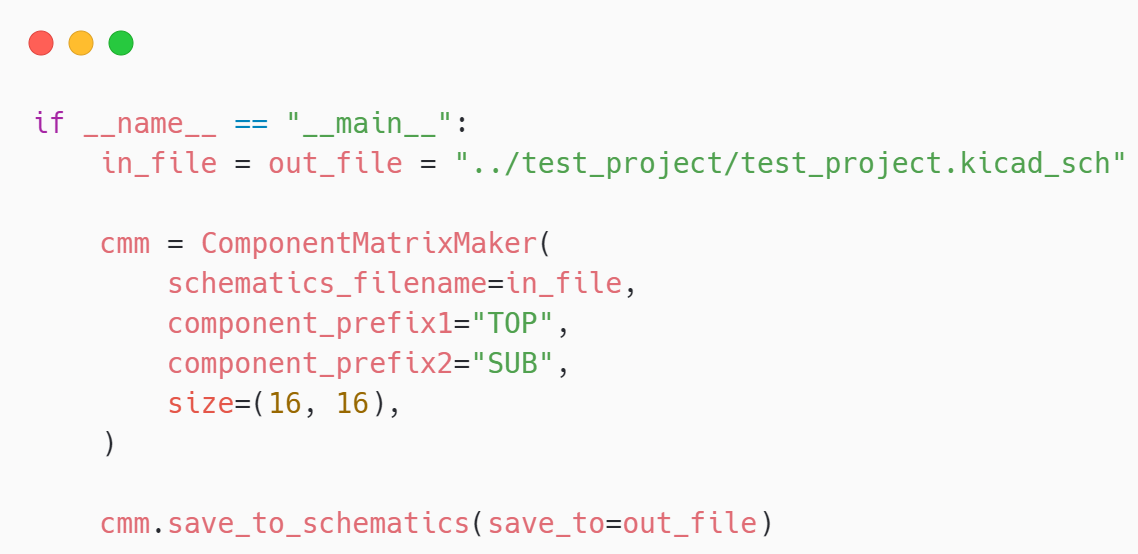
\includegraphics[width=0.8\linewidth]{code_schematics.png}
	\caption[Code to generate Kicad schematic]{Code to generate Kicad schematic}
	\label{fig:coil_schematic}
\end{figure}

\subsection{PCB generation}

Now that we have the schematic, we want to place the coils in a matrix on the PCBnew software. For that, we need to already have exported the components into PCBnew. We also need text files with the list of names of the coils to position.

\begin{figure}[H]
	\centering
	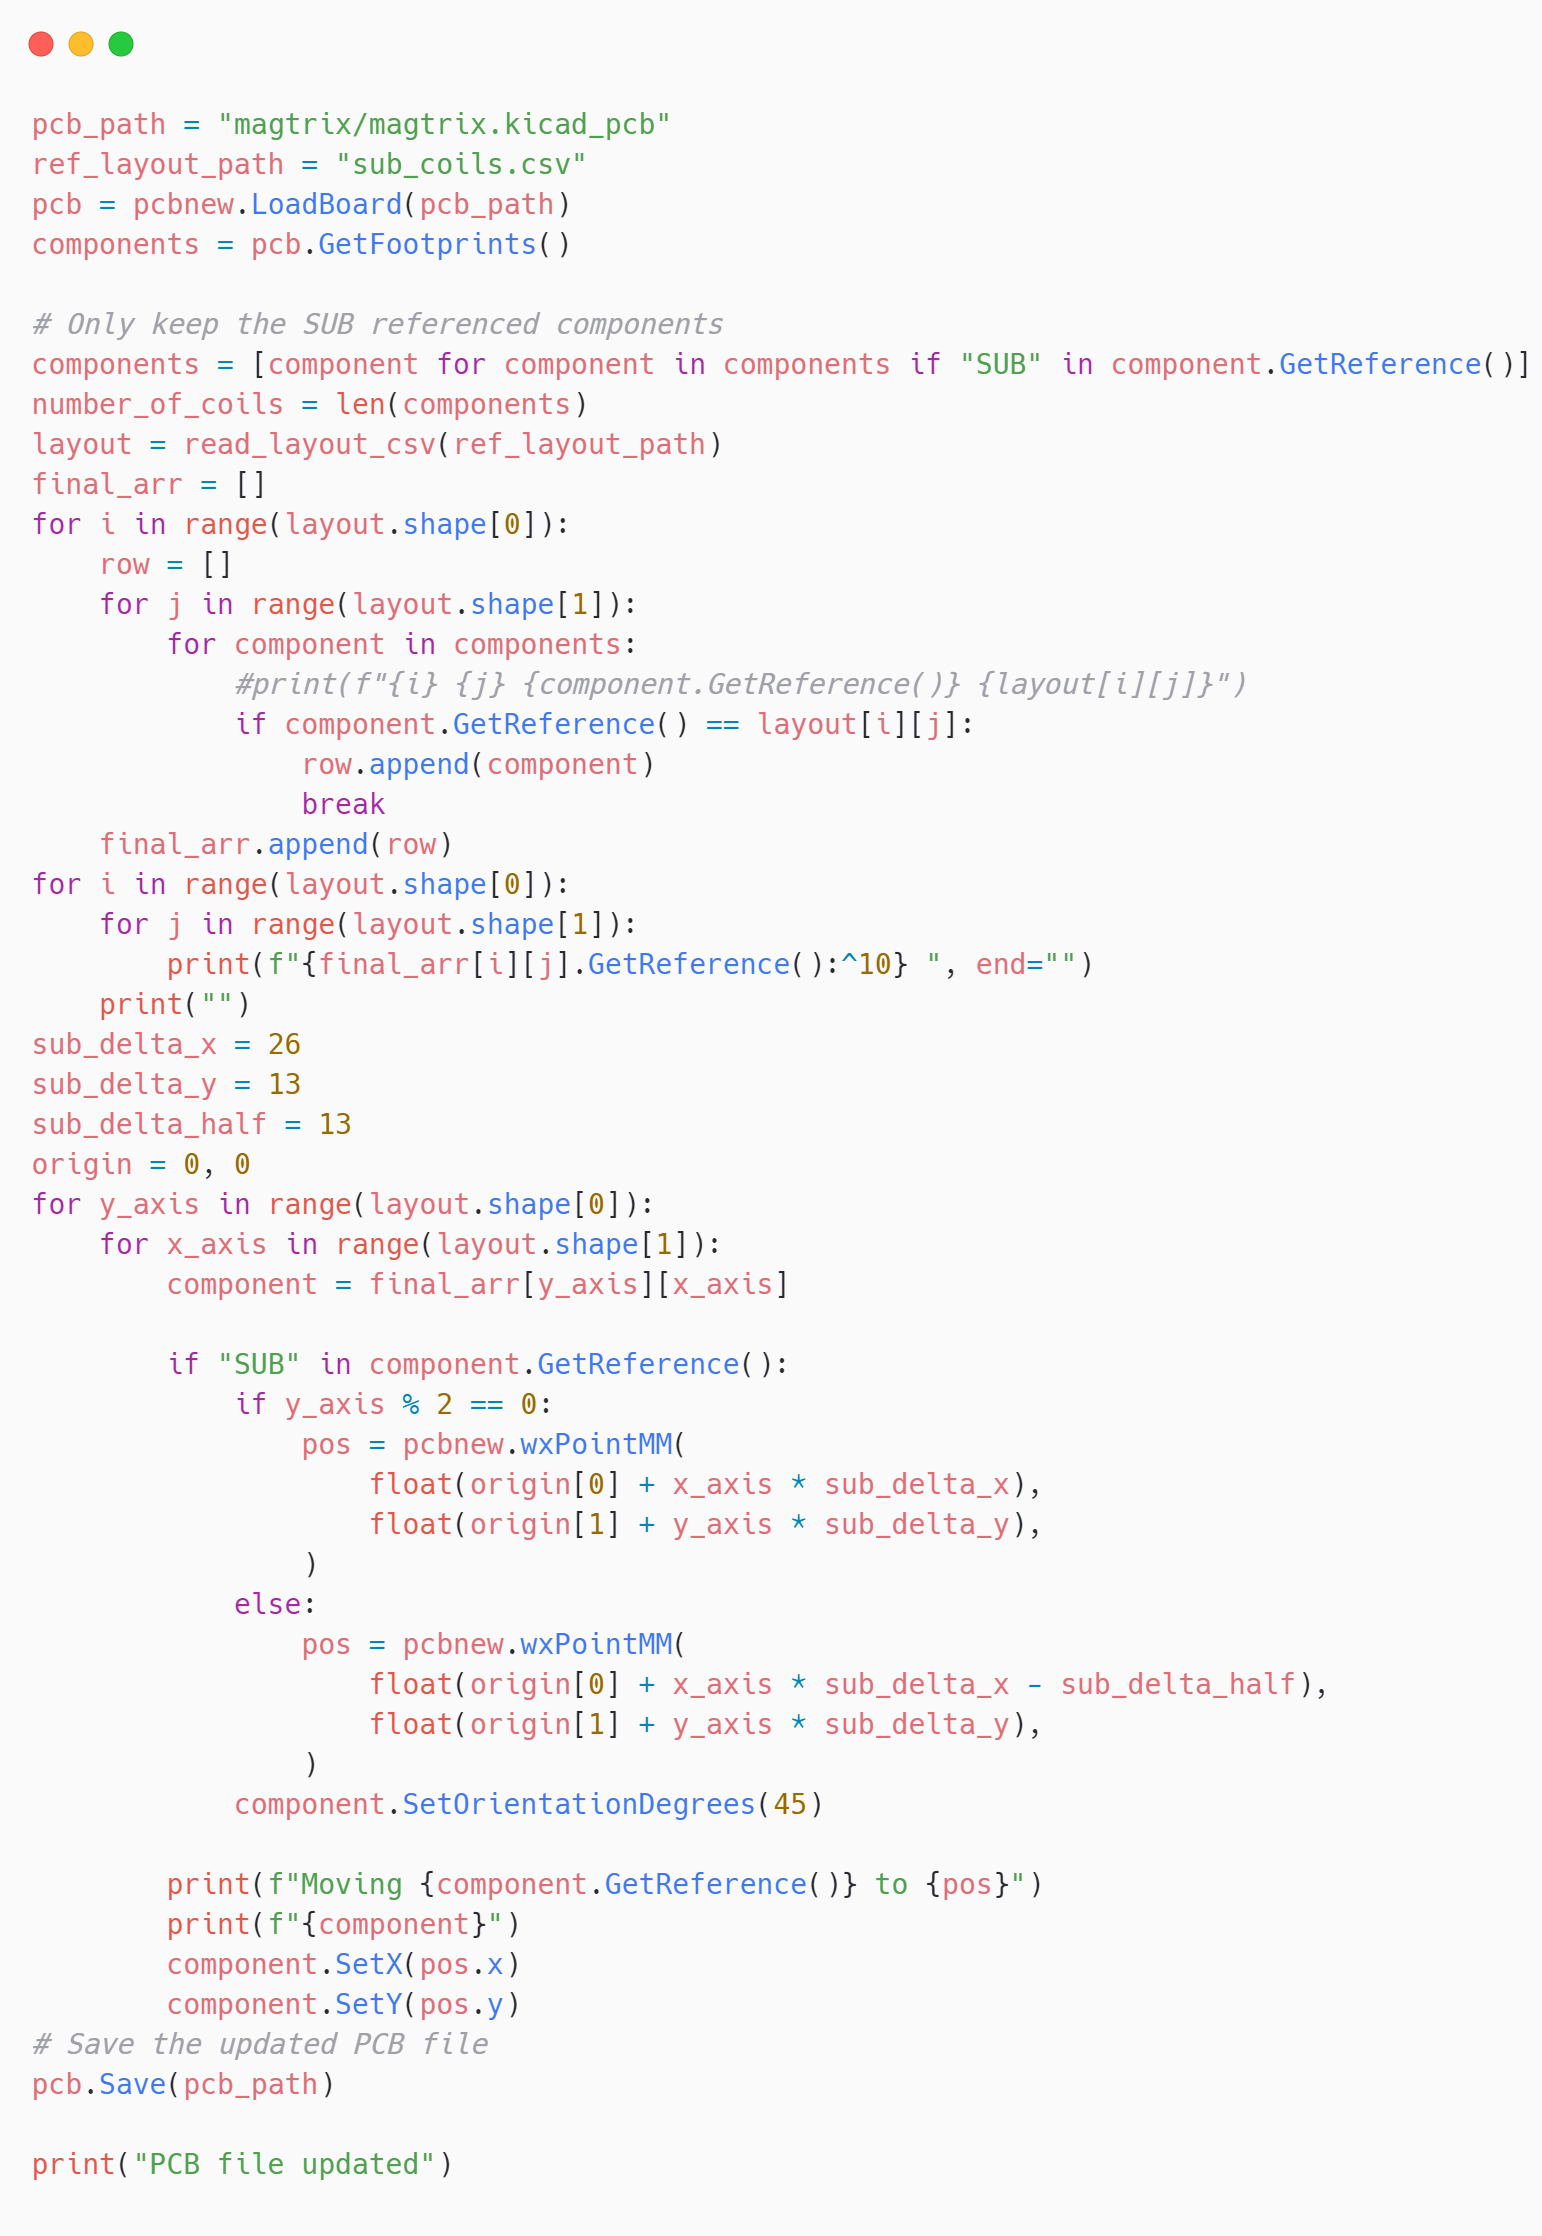
\includegraphics[width=0.8\linewidth]{code_pcb_sub.png}
	\caption[Code to position coils on the PCB]{Code to position coils on the PCB}
	\label{fig:coil_pcb}
\end{figure}

\newpage





\section{Control}

We will use a microcontroller to control the matrix. We integrated the RP2040 microcontroller from Raspberry Pi on the \gls{pcb}. It has enough GPIOs to control each row and column of the matrix and it can produce at least 16 PWM signals from a dedicated peripheral to control the columns NMOS.

\begin{figure}[H]
	\centering
	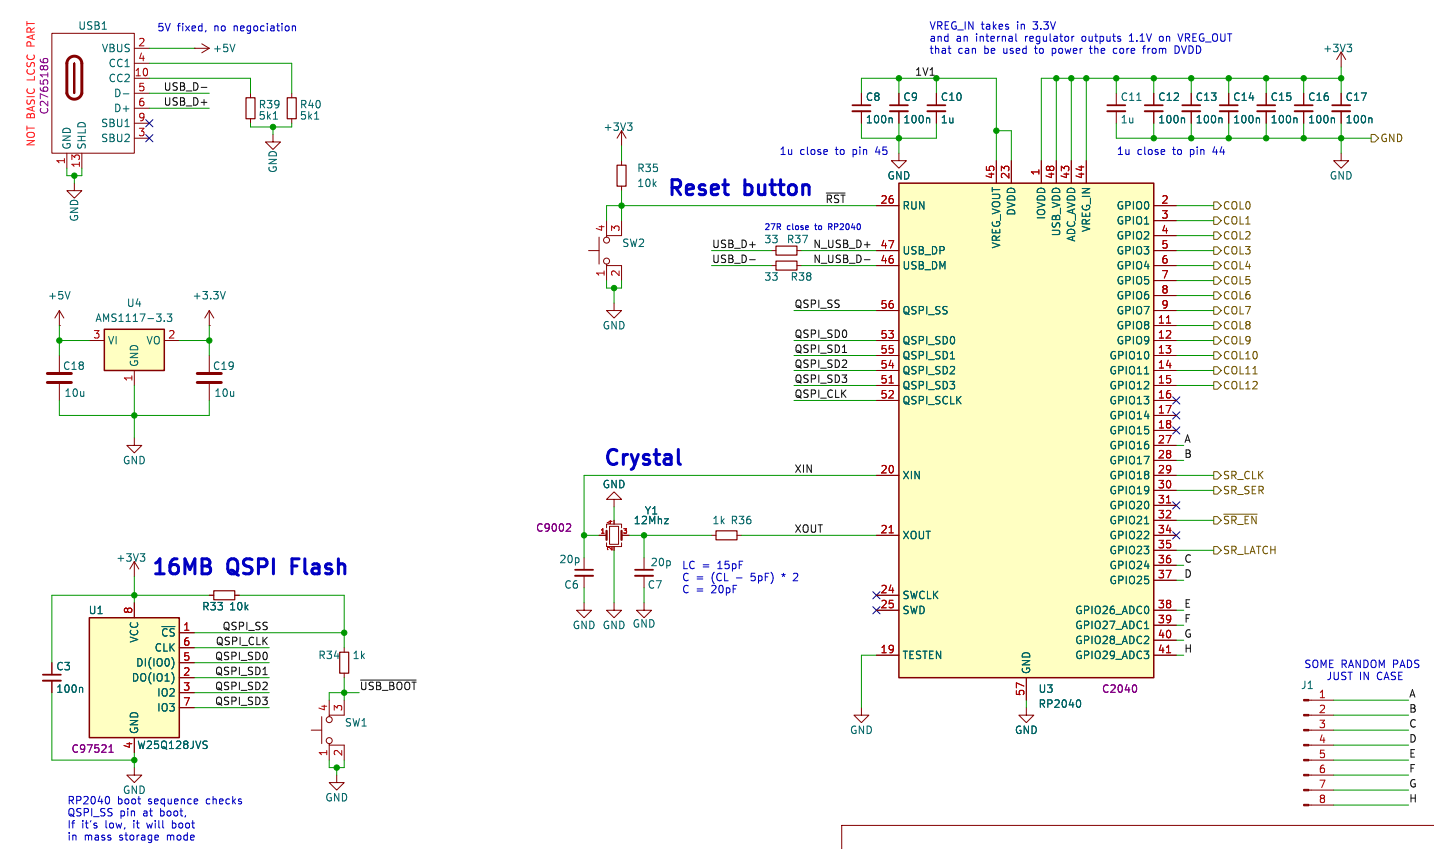
\includegraphics[width=1.5\linewidth, angle=90]{rp2040_schematics.png}
	\caption[RP2040 microcontroller schematics]{RP2040 microcontroller schematics}
	\label{fig:rp2040}
\end{figure}

In order to control bigger matrix, we might have to use a shift reigster to control the rows PMOS, for that purpose, we added a shift register on the \gls{pcb} to future proof the design. Unfortunately, we needed a Serial In Parallel Out shift register with open drain outputs to control the PMOS transistors but I picked the wrong one, so i had to hardwire gpios to the PMOS...

\begin{figure}[H]
	\centering
	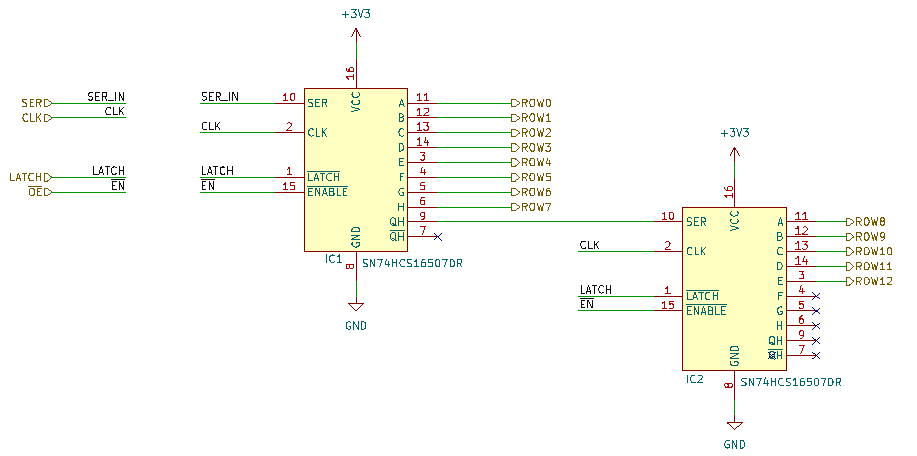
\includegraphics[width=1\linewidth]{shift_registers.png}
	\caption[Shift register schematics]{Shift register schematics}
	\label{fig:shift_registers}
\end{figure}

\newpage

\begin{figure}[H]
	\centering
	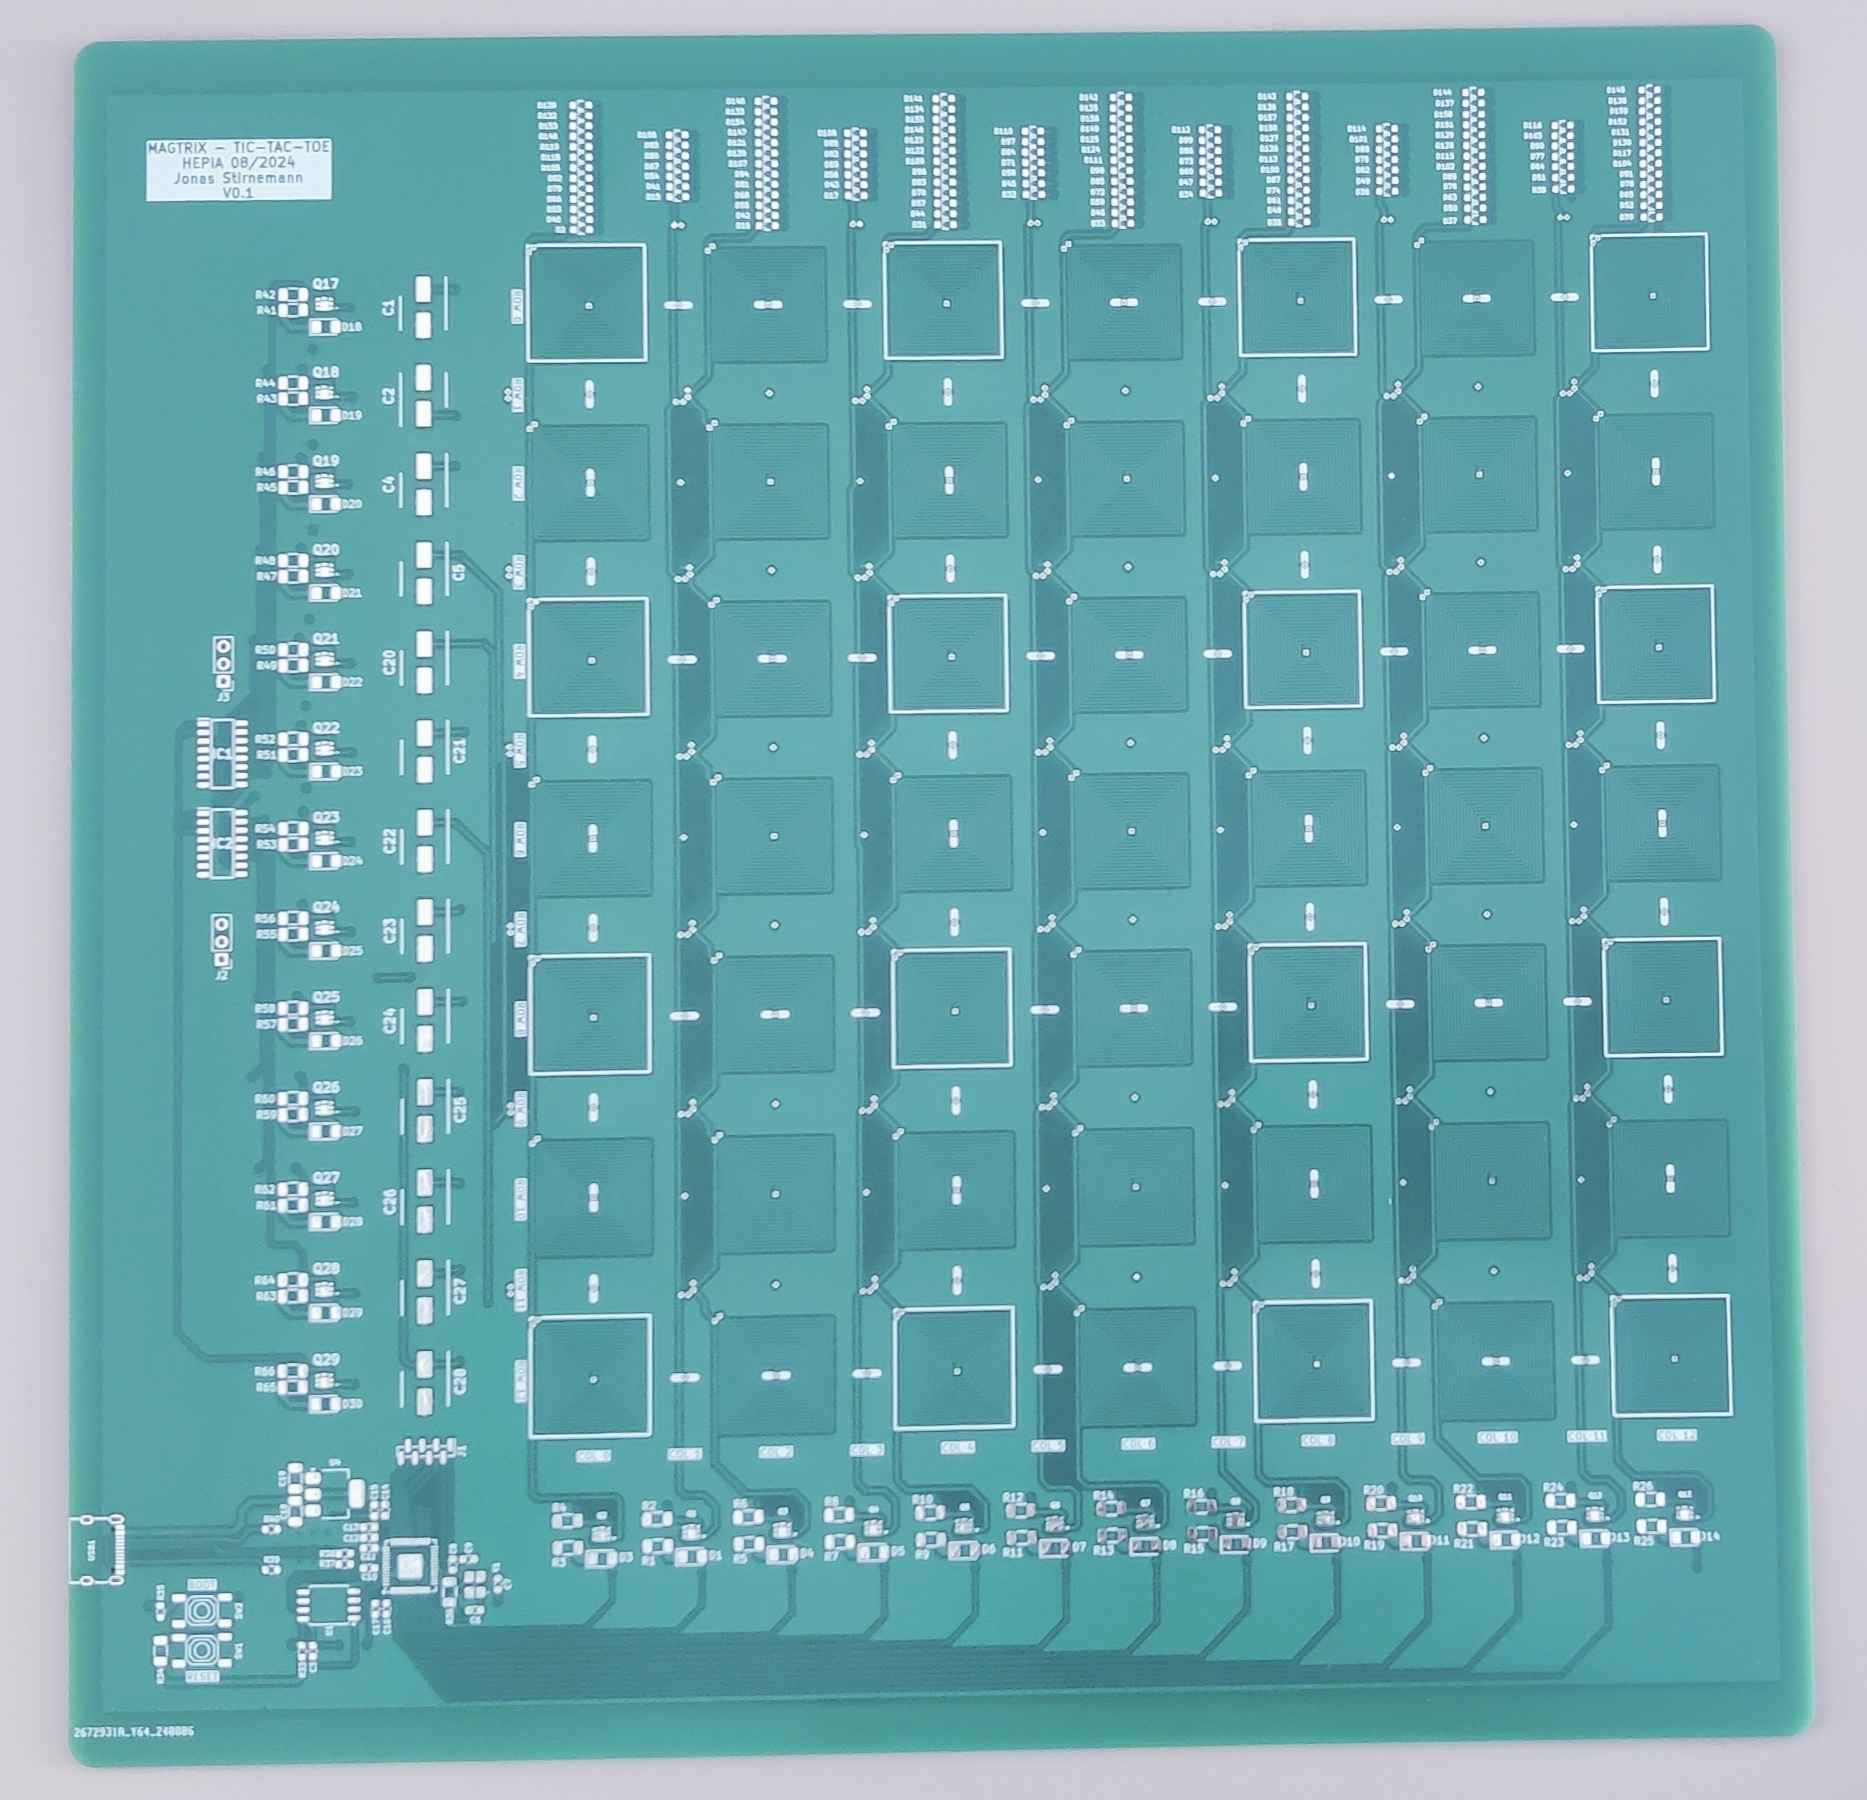
\includegraphics[width=1\linewidth]{final_pcb.jpg}
	\caption[Final Unmounted PCB]{Final Unmounted PCB}
	\label{fig:final_pcb}
\end{figure}

\newpage

The shift registers had to be removed and some gpios were hardwired to the PMOS transistors. We outputed some pads with the remaining free gpios to have some slack in case of issues (Like a wrong Shift register...).

\begin{figure}[H]
	\centering
	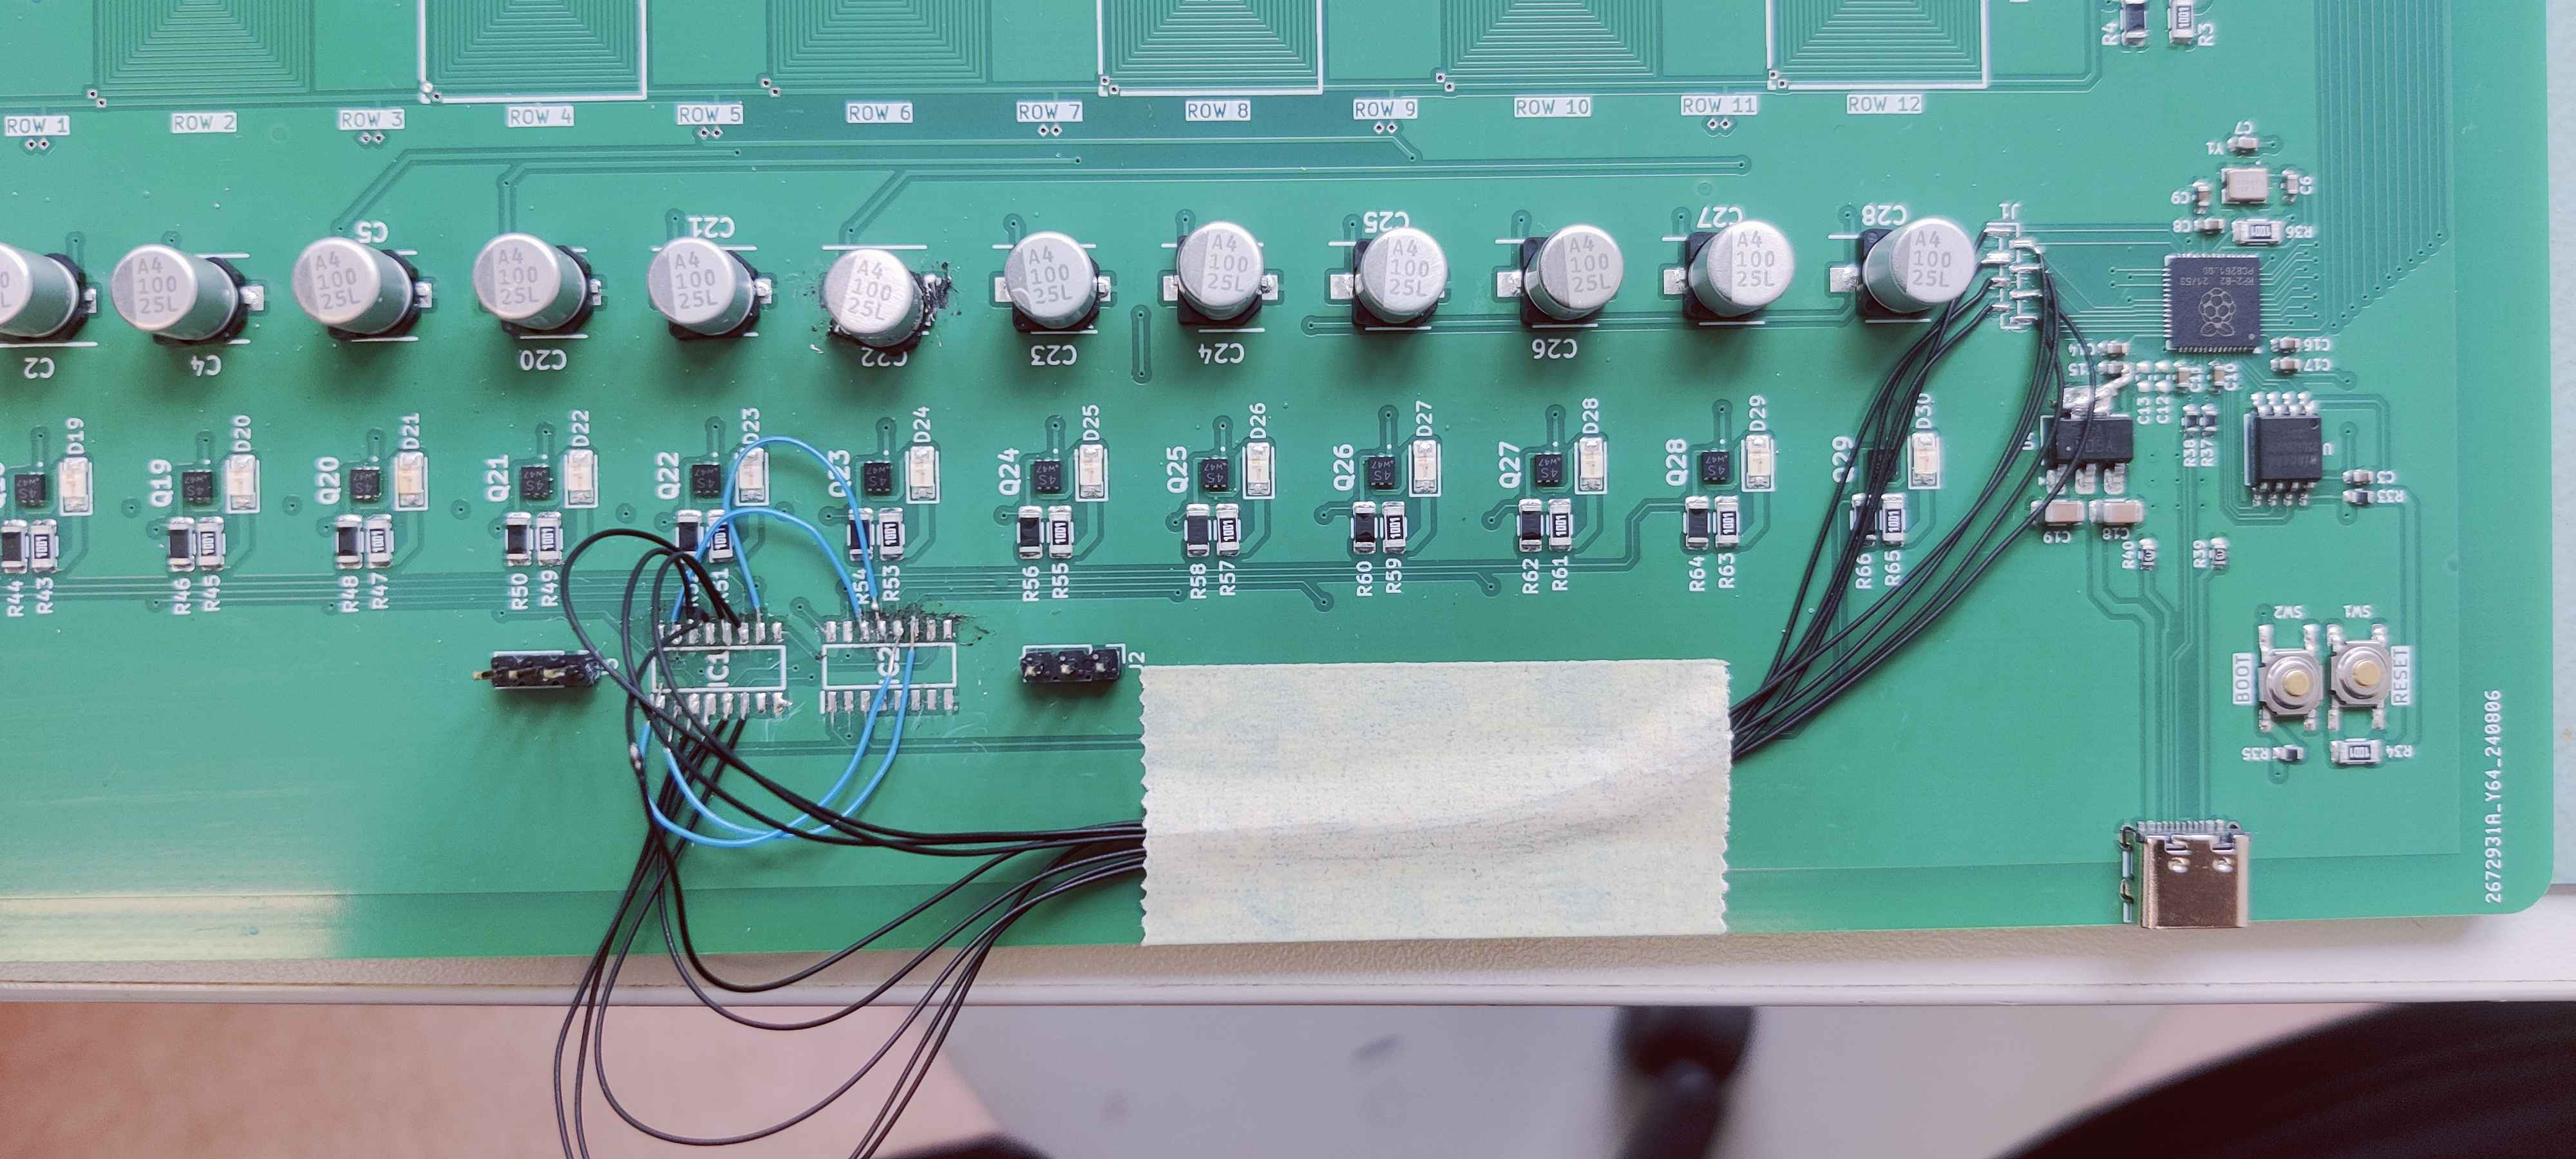
\includegraphics[width=1\linewidth]{ugly_hardware_patch.jpg}
	\caption[Hardware Shift registers fixes]{Hardware Shift registers fixes}
	\label{fig:ugly_hardware_patch}
\end{figure}